\chapter{音の工学的特徴}\label{chap:音の工学的特徴}
\section{\kadaiaa}\label{sec:\kadaiaa}
\purpose 正弦波の生成をプログラミングを用いて作成し,周波数の変化に対して正弦波グラフおよび音の違いを理解する.
\method 時刻\(t\)に対して周波数\(f\)の正弦波は,\eqref{equ:正弦波}で得られる.
\begin{align}
    y & =\sin(2\pi ft)\label{equ:正弦波}
\end{align}
時間軸データ\(t\)を\mat{1}{N}のベクトルに代入する.
時間軸データの作成について,サンプリング周波数\texttt{Fs}に対して\(m\)秒間の正弦波を生成するためには,\ref{src:時間軸作成}のように\texttt{0}から\texttt{Fs}まのベクトルに対して,各要素をサンプリング周波数で割ると時間軸テーブルを作成することができる.\par
\begin{wrapfigure}{r}[0mm]{.4\textwidth}
    \begin{lstlisting}[caption={時間軸作成},numbers={none},label={src:時間軸作成}]
t = (0 : m*(Fs-1)) /Fs;
\end{lstlisting}
\end{wrapfigure}
\(t\)の各要素\(t_n\)に対して三角関数\(\sin(2\pi ft_n)\)を演算し,ベクトル\(y\)の要素\(y_n\)に代入する.従って\(y\)も\mat{1}{N}のベクトルになる.
生成した正弦波を\texttt{plot}関数を用いて\(y\)を\(t\)の関数として描画する.
また,サンプリング周波数を\texttt{Fs}とし,データ列\texttt{y}を再生するためには\texttt{sound}関数を用いる.\par
今回の実験では周波数を\(f_1=440\textrm{Hz}\),\(f_2=660\textrm{Hz}\)の2種類を用いてそれぞれ正弦波\(y_1\),\(y_2\)を生成する.生成した\(y_n(n=\{1,2\})\)に対して,\(t\)を横軸に取りグラフを作成し,サンプリング周波数を\(\textrm{\texttt{Fs}}=16000\textrm{Hz}\)として再生する.\par
\appd{\ref{sec:\kadaiaa}}{src:01_01}
\result 各正弦波のグラフを\ref{fig:\kadaiaa}に示す.音を聴き比べた結果,\(f_2\)の周波数を用いた正弦波は\(f_1\)を用いた正弦波に比べて音が高かった.具体的には\(f_1\)がAの音\footnote{イタリア語音階で「ラ」}であるのに対して,\(f_2\)の音は完全5度大きいEの音\footnote{イタリア語音階で「ミ」}であった.
さらに,聴音確認・目視確認では音の大きさ,音色,振幅や波形の変化は確認でなかった.\par
\begin{wrapfigure}{r}[0mm]{.3\textwidth}
    \caption{周波数が異なる正弦波のグラフ}
    \label{fig:\kadaiaa}
    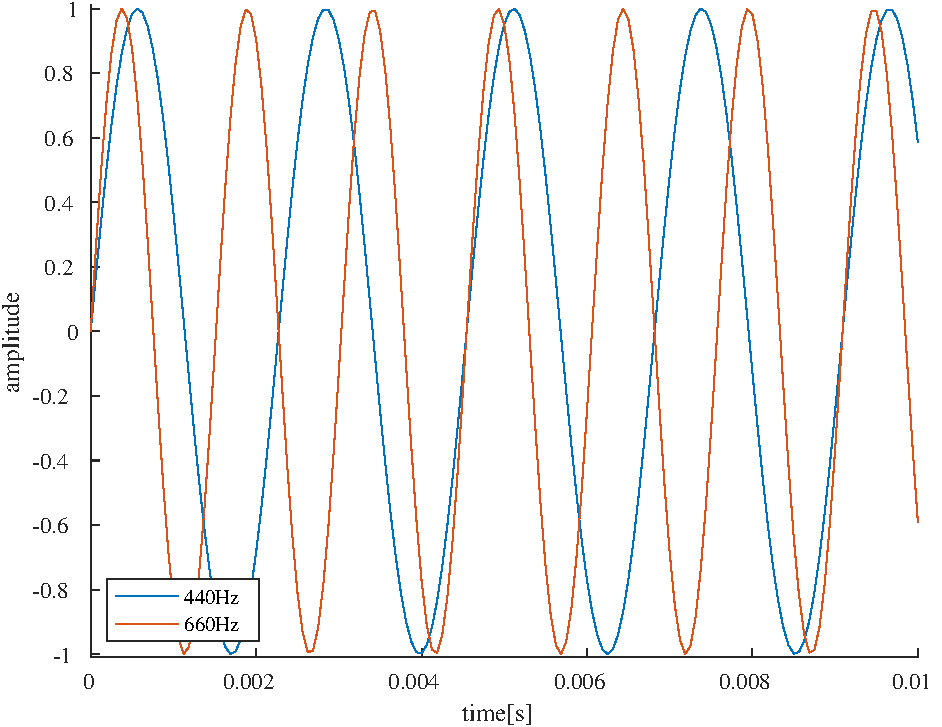
\includegraphics[keepaspectratio,width=.3\textwidth]{../../Figures/01_01.pdf}
\end{wrapfigure}
\consideration 周波数\ \((f)\)\ とは1秒間の振動回数であり,これが音の高さを決める.実験結果より周波数が大きい,つまり1秒間により多く振動すれば音が高くなることが分かった.
また,1回振動あたりの時間を周期\ \((T)\)\ と言うが,周期と周波数は反比例の関係であり,
\begin{align}f & =\frac{1}{T}&\big(\textrm{無論}\quad T\neq 0,\quad f\neq 0\big)\end{align}が成り立つ.\ref{fig:周波数の異なる純音の生成}より,周波数が大きい正弦波は周期が短く,逆もまた確認できる.
周波数のみを変更したので,振幅や正弦波の波形変化はない.
\newpage
\section{\kadaiab}
\purpose 波の振幅や位相を変化させ,変化の前後での音の違いを聞き取り,人間の耳に位相の変化や振幅の変化が聞き取れるかどうか実験し,考察する.
\method 時刻\(t\)に対して周波数\(f\)の正弦波は\eqref{equ:正弦波}で得られるが,その初期位相\footnote{ここでの位相は\textit{phase}を指す.}を\(\phi\)とすると,その正弦波は\eqref{equ:正弦波_位相}となる.
\begin{align}
    y & =\sin(2\pi ft+\phi)\label{equ:正弦波_位相}
\end{align}また,同様な正弦波:\eqref{equ:正弦波}の振幅を\(A\)倍して得られる正弦波は\eqref{equ:正弦波_振幅}となる.
\begin{align}
    y & =A\sin(2\pi ft)\label{equ:正弦波_振幅}
\end{align}この実験では,初期位相の変化と振幅の変化,それぞれ実験し変化前と変化後の音や波形の違いを発見する.周波数は\(f=440\textrm{Hz}\)とする.
\begin{table}[h]
    \caption{\kadaiab の実験内容}
    \label{tbl:\kadaiab_実験内容}
    \begin{tabularx}{\textwidth}{RCCR}
        \multicolumn{1}{c}{\textbf{実験対象}} & \multicolumn{1}{c}{\textbf{振幅(基準倍)}} & \multicolumn{1}{c}{\textbf{初期位相}} & \multicolumn{1}{c}{\textbf{生成される正弦波}} \\
        \hline
        純音                                & 基準                                   & 基準                                & \(y_0=\sin(2\pi ft)\)                 \\
        \hline
        \multirow{2}{*}{振幅}               & \(0.5\)                              & \(0\)                             & \(y_1=0.5\times\sin(2\pi ft)\)        \\
                                          & \(0.25\)                             & \(0\)                             & \(y_2=0.25\times\sin(2\pi ft)\)       \\
        \hline
        \multirow{2}{*}{初期位相}             & \(1\)                                & \(+\frac{\pi}{2}\)                & \(y_3=\sin(2\pi ft+\frac{\pi}{2})\)   \\
                                          & \(1\)                                & \(+\pi\)                          & \(y_4=\sin(2\pi ft+\pi)\)             \\
        \hline
    \end{tabularx}
\end{table}
\section{\kadaiac}
\paragraph{実験の目的}周波数の違いによるうなりの発生やその原因を数学的観点から考察する.
\section{フーリエ級数展開}
\paragraph{実験の目的}フーリエ級数展開を用いた矩形波の描画やフーリエ級数展開のプログラム上での実現性の考察を行う.
\section{白色ガウス雑音}
\paragraph{実験の目的}